\newpage
\chapter{Transient flamelet}
\section{Introduction}
The transient flamelet model of Camflow solves the flamelets equations in mixture fraction coordinate. The model solves the species profiles and the temperature profile as a function of time and mixture fraction.
\section{Fundamentals}
The mass of all atoms of $j$ in a system can be written as
\begin{equation}
 m_j = \sum_{k=1}^{K_g} n_ka_{kj}W_j = \sum_{k=1}^{K_g} \frac{m_k}{W_k}a_{kj}W_j,
\end{equation}
where, $K_g$ is the number of species, $n_k$ the number of moles of species $k$, $a_{kj}$ is the number of atoms pf element $j$ in species $k$, $W_j$ is the atomic mass of element $j$, $W_k$ is the molecular weight of species $k$, and $m_k$ is the mass of species $k$. Mass fraction of element $j$ can be written as 
\begin{equation}
 Z_j = \frac{m_j}{m} = \sum_{k=1}^{K_g} \frac{m_k}{W_k}a_{kj} W_j/m = \sum_{k=1}^{K_g} a_{kj}\frac{W_j}{W_k}Y_k
\label{mixfrac}
\end{equation}
Mass fraction $Y_k$ can be converted to mole fractions $X_k$ according to
\begin{equation}
 Y_k = \frac{X_kW_k}{\bar{W}}
\label{mass2mole}
\end{equation}
substituting \ref{mass2mole} into \ref{mixfrac} gives
\begin{equation}
 Z_j = \frac{W_j}{\bar{W}} \sum_{k=1}^{K_g} a_{kj}X_k, \quad j=1\ldots K_e
\label{mixture_frac}
\end{equation}

Now summing up the mass fractions in the species transport equation defined in \ref{species} and utilizing the relationship \ref{mixfrac} leads to

\begin{equation}
 \frac{\partial }{\partial t}\sum_{k=1}^{K_g} Y_k + \frac{\partial}{\partial x}\sum_{k=1}^{K_g} (\rho u Y_k)+ \frac{\partial}{\partial x} \sum_{k=1}^{K_g} j_kW_k = \sum_{k=1}^{K_g} \dot{\omega}_kW_k 
\end{equation}

 multiplying throughout by $a_{kj}W_j/W_k$ and realizing that the sum over the source term vanishes, the above equation turns to
 \begin{equation}
  \rho \frac{\partial}{\partial t}\sum_{k=1}^{K_g} a_{kj} \frac{W_j}{W_k}Y_k + 
  \rho u \frac{\partial}{\partial x}\sum_{k=1}^{K_g} a_{kj} \frac{W_j}{W_k}Y_k +
 \frac{\partial}{\partial x}\sum_{k=1}^{K_g} a_{kj} \frac{W_j}{W_k}J_kW_k = 0
 \end{equation}
 
substituting  \ref{mixture_frac} into the above equation gives
\begin{equation}
 \rho \frac{\partial Z_j}{\partial t} + \frac{\partial (\rho u Z_j) }{\partial x} + \frac{\partial }{\partial x} \sum_{k=1}^{K_g} a_{kj}\frac{W_j}{W_k}j_kW_k=0, \quad j=1\ldots K_e
\label{conserve_mix_frac}
\end{equation}

\subsection{Diffusion term simplification}
The flux $j_k$ is defined as
\begin{equation}
 j_k = -\frac{\rho D_km}{W_k}\frac{dY_k}{dx}
\label{flux}
\end{equation}

If the diffusion coefficient of all species are assumed to be the same then the 3rd term of Eq.\ref{conserve_mix_frac} can be simplified by the use of Eq.\ref{flux} as
\begin{equation}
 \frac{\partial }{\partial x}\sum_{k=1}^{K_g} a_{kj} \frac{W_j}{W_k}j_kW_k = \frac{\partial }{\partial x}\rho \mathcal{D} \frac{\partial }{\partial x}\sum_{k=1}^{K_g} a_{kj} \frac{W_j}{W_k}Y_k = \frac{\partial }{\partial x}\rho \mathcal{D} \frac{\partial Z_j}{\partial x}
\label{diff_eq_1}
\end{equation}
substituting Eq.\ref{diff_eq_1} back to Eq.~\ref{conserve_mix_frac} gives
\begin{equation}
 \rho \frac{\partial Z_j}{\partial t} + \frac{\partial (\rho u Z_j)}{\partial x} + \frac{\partial}{\partial x}\mathcal{J}_j = 0
\label{diff_eq_2}
\end{equation}
where 
\begin{equation}
 \mathcal{J}_j = \frac{\lambda}{c_p}\frac{\partial Z_j}{\partial x}
\end{equation}

 An equation similar to Eq.~\ref{diff_eq_2} can be derived for mixture fraction $Z$. The mass fraction of the fuel is basically the sum of element mass fractions, i.e
\begin{equation}
 Y_{fm} = \sum_{j=1}^{K_e} Z_{jf}
\end{equation}
The mixture fraction of fuel is defined as 
\begin{equation}
 Z = \frac{Y_{fm}}{Y_{f1}} = \frac{\sum_{j=1}^{K_e}Z_{if}}{Y_{f1}}
\end{equation}
Now a summation over Eq.\ref{conserve_mix_frac} leads to

\begin{equation}
 \rho \frac{\partial Z}{\partial t} + 
\frac{\partial (\rho u Z)}{\partial x} + \frac{\partial }{\partial x}\bigg(\frac{\lambda}{c_p} \frac{\partial Z}{\partial x} \bigg) =0
\end{equation}

\subsection{Transformation to mixture fraction coordinates}
Applying the following transformation rule
\begin{equation}
 \frac{\partial}{\partial x}= \frac{\partial Z}{\partial x} \frac{\partial }{\partial Z}
\end{equation}
to energy equation Eq.~\ref{energy} leads to


\begin{equation}
\begin{split}
 \rho \partialfrac{T}{t} + \rho u \partialfrac{Z}{x}\partialfrac{T}{Z} - \frac{\lambda}{c_p}\partialfrac{Z}{x}\partialfrac{{^2Z}}{{x\partial Z}} \partialfrac{T}{Z} -
\frac{\lambda}{c_p}\bigg( \partialfrac{Z}{x}\bigg)^2 \partialfrac{{^2T}}{{Z^2}} + \\
\frac{1}{c_p}\sum_{k=1}^{K_g} c_{pk	} \partialfrac{Z}{x}\partialfrac{T}{Z}\rho\mathcal{D}\partialfrac{Z}{x}\partialfrac{{Y_k}}{Z} + 
\frac{1}{c_p} \sum_{k=1}^{K_g} h_k\dot{\omega}_k = 0
\end{split}
\end{equation}
Now if the flamelet is thin in the $Z$ direction an order of magnitude analysis shows that the second derivative with respect to $Z$ is the dominating term, leading to the simplified form of the above equation as
\begin{equation}
 \rho \partialfrac{T}{t} -\frac{\lambda}{c_p}\bigg( \partialfrac{Z}{x} \bigg)^2 \partialfrac{{^2T}}{{Z^2}}
+ \frac{\rho \mathcal{D}}{c_p} \bigg(\partialfrac{Z}{x}\bigg)^2 \bigg[\sum_{k=1}^{K_g}c_{pk}\partialfrac{{Y_k}}{Z}\bigg] \partialfrac{T}{Z} + \frac{1}{c_p}\sum_{k=1}^{K_g} h_k\dot{\omega}_k = 0
\label{T_mixfrac}
\end{equation}
Defining the scalar dissipation rate ($\chi$) as
\begin{equation}
 \chi = 2\mathcal{D} \bigg( \partialfrac{Z}{x} \bigg)^2,
\end{equation}
and assuming unit Lewis number and the same specific heat capacity for all species simplifies Eq.~\ref{T_mixfrac} to

\begin{equation}
 \rho \partialfrac{T}{t} - \frac{\rho \chi}{2}\partialfrac{{^2T}}{{Z^2}} + \frac{1}{c_p} \sum_{k=1}^{K_g} h_k\dot{\omega}_k =0
\end{equation}

Applying the same procedure to the species transport equation~\ref{species} gives
\begin{equation}
 \rho \partialfrac{{Y_k}}{t} - \frac{\rho \chi}{2}\partialfrac{{^2Y_k}}{{Z^2}} = \dot{\omega}_k W_k
\end{equation}

The scalar dissipation rate $\chi$ is related to the strain rate $a$ in a counter flow flame by
\begin{equation}
 \chi = \frac{a \exp \bigg( -2[\mathrm{erfc}^{-1}(2Z)]^2 \bigg)} {\pi},
\end{equation}
where $Z$ is the mixture fraction

 \section{Input file}
An example of ``camflow.xml'' input file for flamelet is shown below
{\scriptsize{
\begin{verbatim}
<?xml version="1.0" encoding="ISO-8859-1"?>
<camflow>
   <reactor model="flamelet">
    <length unit="cm">1.0</length>
  </reactor>
  <op_condition>
     <temperature>adiabatic</temperature>
     <pressure unit="bar">1</pressure>
     <strain>400</strain>
  </op_condition>
  <inlet>
     <fuel>
       <velocity unit="m/s">1.0</velocity>
       <temperature unit="K">300.0</temperature>
       <molefrac>
        <species name="H2">1.0</species>
       </molefrac>
     </fuel>
     <oxidizer>
       <velocity unit="m/s">1.0</velocity>
       <temperature unit="K">300.0</temperature>
       <molefrac>
        <species name="O2">0.21</species>
        <species name="N2">*</species>
       </molefrac>
     </oxidizer>
  </inlet>
  <solver mode="coupled" solver="cvode" residual="on">
     <maxTime>10000</maxTime>
     <iterations>1</iterations>
     <tols>
        <species>
           <aTol>1.e-12</aTol>
           <rTol>1.e-08</rTol>
        </species>
        <temperature>
           <aTol>1.e-03</aTol>
           <rTol>1.e-03</rTol>
        </temperature>
        <flow>
           <aTol>1.e-03</aTol>
           <rTol>1.e-03</rTol>
        </flow>
     </tols>
  </solver>
  <initialize>
    <mCenter unit="cm">50</mCenter>
    <mWidth unit="cm">40</mWidth>
    <massfrac>
      <intrmdt name="H">0.1</intrmdt>
    </massfrac>    
 </initialize>
 <report outfile="final" species="mole">
 </report>
 <grid>grid.inp</grid>
</camflow>

\end{verbatim}}
}

The input file follows xml standard. A detailed description about the various elements in the input file is specified below.

\begin{itemize}
 \item \textbf{rector} : The reactor element specifies which model is to be simulated and for flamlet camflow expects ``flamelet'' as the model attribute value. The reactor element also holds child element length for specifying the nozzle separation, and is given with the unit attribute. Since the flamelet equations are solved in the mixture fraction coordinate, this element has no meaning in this case.

\item \textbf{op\_conditions} : The element op\_conditions describes the operating conditions for the flame. This includes the specification of the pressure and the condition applied to the solution of energy equation. The flame pressure may be specified in the units of ``Pa'', ``atm'', or ``bar''. The temperature element can take the values of ``isothermal'', ``adiabatic'', or ``userdefined''. However, for flamelets the option should either be adiabatic or userdefined.\\

In addition to the temperature and pressure, the strain rate needs to be specified for the calculation of scalar dissipation rate.

\item \textbf{inlet} : For flamelets there are two inlets; one for the fuel and the other for the oxidizer. All properties pertaining to the fuel inlet must be specified under the element ``fuel'' and all properties pertaining to the oxidizer inlet must be specified under the ``oxidizer'' element. Both ``fuel'' and ``oxidizer'' element must specify the velocity at the inlet using the ``velocity'' element, temperature using the ``temperature'' element and the species composition using ``molefrac'' or ``massfrac'' element.The unit for velocity may be in m/s or in cm/s and temperature can be in C or in K. The appropriate units must be specified as attribute values. The chemical species present in the fuel/oxidizer can be specified using the species elements, with the species name as attribute and corresponding mole/mass fraction as attribute. The last species composition may be specified using ``*'', and this case the ``*'' will stand for 1-sum of composition of other species. 

\item \textbf{solver}: The solver element holds the solver control specifications. The attributes ``mode'' can be specified as ``coupled'' or ``segregated'' for flamelets. The solver name is essentially provided to switch from one solver to another. However, the present version of Camflow uses only CVode as the numerical integrator, and therefore accepts only ``cvode'' as the solver name. When the solver mode is specified as coupled, the governing equations are solved simultaneously, and for ``segregated'' mode, the governing equations are solved sequentially for a number of times that is specified by the element integrations. By default the value of iterations element is one. At the end of the number of iterations, the solution mode will automatically switch to coupled. The user is encouraged to use coupled mode for flamelet calculations.\\

Additionally the integration time may be optionally specified by the element maxTime. By default the value of maxTime is 100000 s. However, the final integration time is the maxTime or the time required to reach steady state whichever is lower. This means the solver will stop integration, if steady state is reached before the specified integration time.\\

The element ``tols'' hold the various tolarences that can be applied to the species, energy, and continuity equations. For species a relative tolerance of at least 10$^{-6}$ should be used. The user may need to adjust the tolarence values for the species in case of solution difficulties.

\item \textbf{initialize} The initialize element can be used to specify various initial conditions. 
A guess value for the intermediate species composition has to be specified to initialize the flow filed. When specifying the intermediate compostions, the mixing center and mixing width needs to be specified. When these compositions are specified a guassien profile will be generated for the intermediate species with peaks at the mixing centers and the having the spread specified by mixing width. The mixing center is specified by the element ``mCenter`` and the mixing width is specified by ''mWidth``. Both these elements are provided with ''unit`` attribute, and appropriate unit of length must be specified. Unlike the specification of fuel inlet species composition, the sum of intermediate or product species composition need not to sum up to one. However, the user must ensure that the sum does not exceeds one.\\

The temperature profile can be specified by using the ``Tprofile'' element with two attributes namely ``unit\_L'' for length unit and ``unit\_T'' for temperature unit. The length unit can be in ``cm'' or in ``m'', where as the temperature unit can be either in ``K'' or in ``C''. The actual temperature as a function of reactor position is specified with the child elements position with the attribute ``x'', which stands for the position with the reactor. If the length unit is specified as ``cm'' then ``x'' is the position from the reactor inlet in ``cm'', and the value for the position element is the temperature at position ``x''. However, this is not mandatory.

\item \textbf{report}: The desired output for the species composition must be specified in this element using the species attribute. ``mole'' or ``mass'' may be used as the attribute values, and correspondingly the output will be produced either in mole fraction or mass fractions.

\item \textbf{grid}: The flamelet model requires a discretized geometry in the mixture fraction coordinate. The geometry may be specified using anyfile that contains a nodes of the descretised mixture fraction coordinate. In the case of flamelets the contents of the grid file does not have any units are they are simply mixture fraction coordinates at which the solution is desired. An example is shown below\\
{\scriptsize{\begin{verbatim}
0.0
0.002
0.003
0.004
0.005
0.006
0.007
0.009
0.01
0.015
0.02
0.03
0.04
0.05
0.06
0.07
0.08
0.09
0.1
\end{verbatim}
}}

\end{itemize}

\section{Executing the binary}
The flamelet model of Camflow expects four input files namely, ``camflow.xml'', ``therm.dat'',  ``chem.inp'', and ``tran.dat''. All the files must be present in the working directory. Upon successful execution the output file ``profile.dat'' containing the final integration time (s), mixture fraction, scalar dissipation rate (1/s), density (kg/m$^3$), temperature (K), and the species compositions in mass or mole fractions.

\section{Results}
Fugure~\ref{flamelet_profile} show the steady state profiles of various chemical species as a function of mizture fraction coordinate with both fuel and oxidizer entering at 300 K, and Fig.~\ref{flamelet_temp} shows the temperature profile as a function of mixture fraction.

\begin{figure*}[h]
 \centering
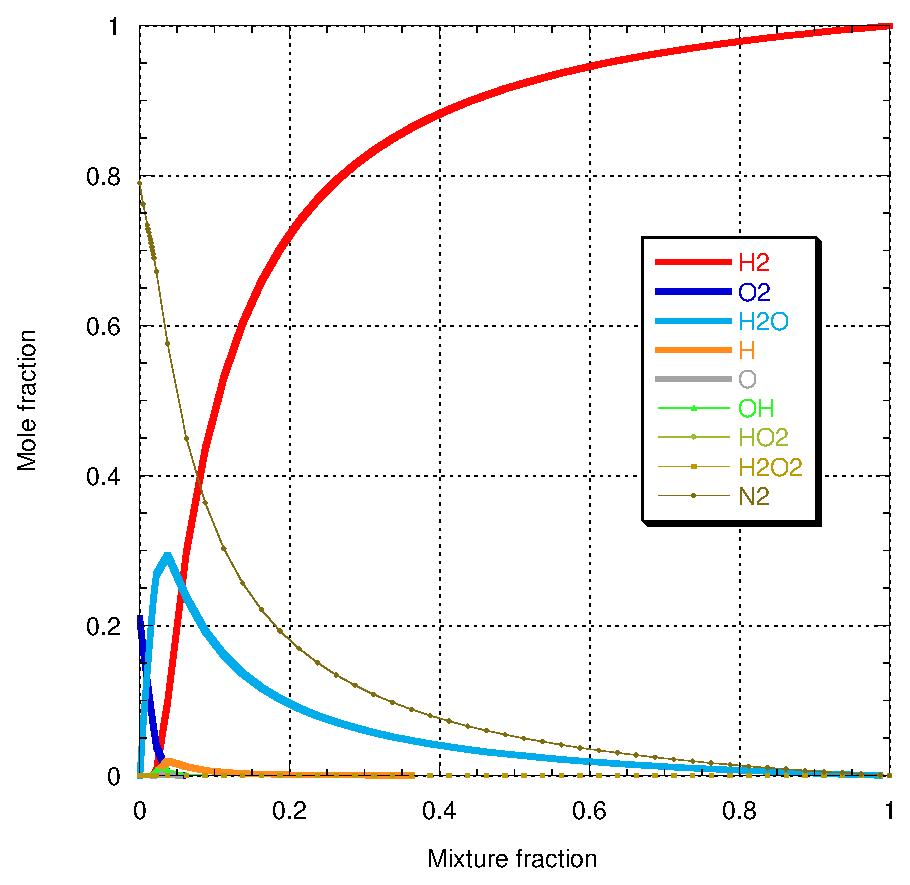
\includegraphics[scale=0.6]{flamelet_profile.eps}
\caption{Species profile for hydrogen flame}
\label{flamelet_profile}
\end{figure*}

\begin{figure*}[h]
 \centering
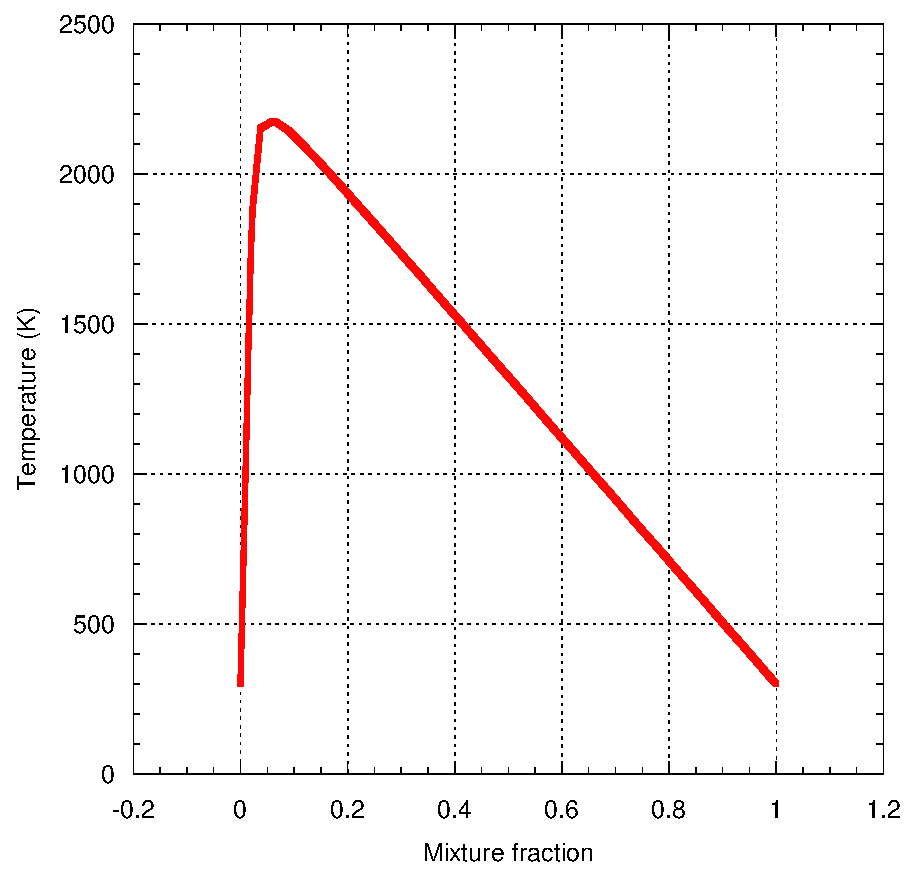
\includegraphics[scale=0.6]{flamelet_temp.eps}
\caption{Temperature profile for hydrogen flame}
\label{flamelet_temp}
\end{figure*}

%===============================================================================================
%
%
%
%===============================================================================================
